% -*- mode: LaTeX; coding: utf8; -*-

\documentclass[a4paper,12pt]{extreport}

% правильне кодування
\usepackage[T2A]{fontenc}
\usepackage[utf8]{inputenc}
\usepackage[ukrainian]{babel}


% починати абзаци невеликим відступом першого рядка
\usepackage{indentfirst}
\usepackage[pdftex,unicode,bookmarks]{hyperref}

\usepackage{color}
\definecolor{bluegray}{RGB}{230,230,255}
\usepackage{listings}

\usepackage{algorithmicx}

\lstset{
	extendedchars=\true, % дозволити кирилицю в лінстингу
	inputencoding=utf8,
	breaklines=true,
	basicstyle=\ttfamily,
	numbers=left,
	frame=single,
	backgroundcolor=\color{bluegray}
}

% якщо прийдеться вставляти код (простіше ніж listings, але немає breaklines)
\usepackage{verbatim}

% інтервал - півтора. 
\usepackage{setspace}
\onehalfspacing

% поля
\usepackage{geometry}
\geometry{a4paper}
\geometry{left=35mm,right=15mm,top=20mm,bottom=20mm}
\geometry{headheight=2ex,headsep=10mm,footskip=10mm}

%
\usepackage{mathtools}
\usepackage{mathrsfs, amsmath}

%для картинок
\usepackage{graphicx}
\usepackage{caption}

% lstlisting settings
\usepackage{xcolor}

% для часткових похідних
\usepackage{physics}


% для алгоритмів
%\usepackage[ruled,vlined]{algorithm2e}
\usepackage{algpseudocode}
\usepackage{algorithm}
\floatname{algorithm}{Algorithm}
\renewcommand{\algorithmicrequire}{\textbf{Input: }}
\renewcommand{\algorithmicensure}{\textbf{Output: }}
\newcommand{\algorithmreturn}{\textbf{return }}

\definecolor{codegreen}{rgb}{0,0.6,0}
\definecolor{codegray}{rgb}{0.5,0.5,0.5}
\definecolor{codepurple}{rgb}{0.58,0,0.82}
\definecolor{backcolour}{rgb}{0.95,0.95,0.92}

\lstdefinestyle{mystyle}{
	backgroundcolor=\color{backcolour},   
	commentstyle=\color{codegreen},
	keywordstyle=\color{magenta},
	numberstyle=\tiny\color{codegray},
	stringstyle=\color{codepurple},
	basicstyle=\ttfamily\footnotesize,
	breakatwhitespace=false,         
	breaklines=true,                 
	captionpos=b,                    
	keepspaces=true,                 
	numbers=left,                    
	numbersep=5pt,                  
	showspaces=false,                
	showstringspaces=false,
	showtabs=false,                  
	tabsize=2
}
\lstset{style=mystyle}

% bibliography
\usepackage[
backend=biber,
style=numeric,
sorting=ynt
]{biblatex}
\addbibresource{resources/bibres.bib}

% custom commands
\newcommand{\tran}{^{T}}
\newcommand{\ith}{^{(i)}}



\begin{document}
	% ============================================ %
	\begin{titlepage}%
    	\begin{center}
	    	\large{\textbf{ЛЬВІВСЬКИЙ НАЦІОНАЛЬНИЙ УНІВЕРСИТЕТ \\ ІМЕНІ ІВАНА ФРАНКА}}\par
	       	{Факультет прикладної математики та інформатики\\ Кафедра обчислювальної математики}\par
			\begin{center}
	
	        \end{center}
	        \vspace{25mm}
	        \textbf{\Huge{Курcова робота}}\par
	        \vspace{5mm}
	        {\large{АНАЛІЗ АТАК НА ЛІНІЙНІ МОДЕЛІ МАШИННОГО НАВЧАННЯ}}\par
	        \vspace{5mm}
	        {}\par %subtitle
        \end{center}
	   	
	   	\vspace{30mm}
	   	
		\begin{flushright}
   	   		\begin{minipage}[t]{100mm}
   	   			\flushleft
   	   			\large{
	   	   		Виконав: студент \underline{III} курсу групи \underline{ПМп-31} напрямку підготовки (спеціальності) \\
	   	   		123 $-$ "Прикладна математика" \hfill \\
				}
	   	   	   	\large{	   	   	   			   	   		\noindent\underline{\makebox[100mm]{\hfill Середович В.В.}} \\
   	   			}
      			\small{
	   	   		\hfill \footnotesize{(прізвище та ініціали)} \\
	   	   		}
	   	   		\large{
	   	   			Керівник: \noindent\underline{\makebox[76.5mm]{\hfill Музичук Ю.А.}}
   	   			} \\
	   	   		\small{
	   	   		\hfill \footnotesize{(прізвище та ініціали)} \\
	   	   		\vspace{2ex}
				}
   	   		\end{minipage}
   	   \end{flushright}
	   \vfill
   	   
   	   \begin{center}Львів --- 2020\end{center}
   	   \stepcounter{page}
    \end{titlepage}
	% ============================================ %
	
	
	% ============================================ %
	\tableofcontents
	\newpage

	% ============================================ %
	
	
	% ============================================ %
	\chapter{Вступ}
	Алгоритми машинного навчання активно використовується у різних областях нашого життя та дуже добре демонструють себе у задачах класифікації. Однак, виявляється, що ці алгоритми є досить вразливими навіть до незначних, правильно підібраних, пертурбацій вхідної інформації. Такі модифіковані приклади, які навмисно змінють для того, щоб вони були хибно передбаченні називають змагальними прикладами або adversarial samples. В деяких випадках ці зміни можуть бути настільки малі, що для людини вони зовсім не будуть помітні, однак класифікатор моделі буде робити хибне передбачення. Така вразливість може бути дуже небезпечною, коли алгоритми машинного навчання застосовуються в критичних для здоров'я людини середовищах. Саме тому ця область привертає до себе багато уваги і порбеюує досліджень. 
	
	В межах теми цієї роботи будуть розглядатись різні методи атак на лінійні моделі машинного начання які будуть аналізуватись і порівнюватись між собою. Також будуть запропоновані методи захисту моделі.
	
	\section{Постановка задачі} 
	
	\textit{Мета} даної роботи полягає у тому, щоб дослідити ефективність атак на лінійні моделі машинного навчання, та визначити методи захисту від них. \par
	Виходячи з мети, визначені завдання роботи:
	\begin{itemize}
	\item Реалізувати лінійну модель машинного навчання
	\item Дослідити різні методи генерування змагальних прикладів
	\item Проаналізувати ефективнівсть атак
	\item Визначити методів захисту
	\end{itemize}

	
	\section{Основні поняття}
	
	В цій секції будуть розглянуті основні поняття, які будуть використовуватись в ході роботи. 
	
	\textbf{Змагальний приклад (Adversarial sample)}
	\newline
	Нехай існує класифікатор $f(x):x\rightarrow y$, де  $x \in X, y \in Y$, який передбачає значення $y$ для вхідного $x$. Метою змагального прикладу є знайти такий $x^{*}$, який знаходиться в околі $x$, але хибно визначається класифікатором. Зазвичай максимальний рівень шуму який може бути в змагальному прикладі може бути не більше за певну $L_p$ норму $ \| x^{*} - x \|_p < \varepsilon $, де $p=1,2,\infty $. В межах даної роботи для визначення рівня пертурбації буде виористовуватись саме $L_{\infty}$ норма.
	\par
	\textbf{Націлені атаки (Untargeted Attacks)} \newline
	Націлені атаками є атаки метою яких є внести в приклад $x$, який правильно передбачається як $f(x) = y$ незначний шум так, щоб класифікатор зробив хибне передбачення $f(x^{*}) \neq y$.
	\par
	\textbf{Ненацілені атаки (Targeted Attacks)} \newline
	Ненацілені атаками називають такі атаки, метою яких є внести у вхідний приклад $x$ такі пертурбації щоб класифікатор передбачив якийсь конкретний клас $f(x^{*}) = y^{*}$, де $y^{*}$ є заданою ціллю $y^{*} \neq y$.
	\par
	\textbf{Атаки на закриту модель (White Box attacks)} \newline
	Атаки на закриту модель описують такий сценарій, коли в нападника є повний доступ до параметрів і градієнтів моделі.
	\par
	\textbf{Атаки на відкриту модель (Black Box attacks)} \newline
	До атак на відкриту модель відносять атаки, при яких в нападника нема доступу до параметрів моделі. 
	% ============================================ %

	% ============================================ %
	\chapter{Модель і датасет}
	
	\section{Мультикласова логістична регресія}
	\label{sec:lg}
	В якості лінійного методу машинного навчання, на котрий будуть сдійснюватись атаки буде використовуватись модифікований алгоритм логістичної регресії для мультикласової класифікації. \par
	Нехай маємо набір тренувальних даних:
	\begin{equation*}
		(x^{(1)}, y^{(1)}), \quad (x^{(2)}, y^{(2)}), \quad ... \quad ,(x^{(m)}, y^{(m)})
	\end{equation*}
	\begin{equation*}
		\quad
		%%%
		X =	
		\begin{bmatrix}
		\vdots  & \vdots  & & \vdots \\
		x^{(1)} & x^{(2)} &   \dots & x^{(m)}\\
		\vdots  & \vdots  & & \vdots
		\end{bmatrix}
		%%%
		\quad
		%%%
		x \in
		\begin{bmatrix}
		x_1   \\
		\dots \\
		x_n
		\end{bmatrix}
		\hspace{21 mm}
		%%%
	\end{equation*}
	\begin{equation*}
		\quad
		%%%
		Y =	
		\begin{bmatrix}
		\vdots  & \vdots  & & \vdots \\
		y^{(1)} & y^{(2)} &   \dots & y^{(m)}\\
		\vdots  & \vdots  & & \vdots
		\end{bmatrix}
		%%%
		\quad
		%%%
		y \in
		\begin{bmatrix}
		y_1   \\
		\dots \\
		y_C
		\end{bmatrix}
		\quad
		y_1, ..., y_C
		%%%
	\end{equation*}
	\newline
	$X$ - матриця в якої кожен стовпець є набором характеристик $i-$ого прикладу, \newline $i=1,\dots,m$ 
	\newline
	$Y$ - матриця класів в якої кожен стовпець це масив розмірності $C$, з одиницею на місті справжнього класу
	\newline
	$m$ - кількість характеристик
	\newline
	$n$ - кількість характеристик в кожному прикладі
	\newline
	$C$ - кількість класів
	\newline \newline
	Задача прикладу $x \in R^{n}$, знайти $\hat{y}=P(y = 1 \mid x), \quad 0 \leq \hat{y} \leq 1$
	\begin{center}
	%Шукатимемо у вигляді:
	$\hat{y} = softmax(\omega\tran x + b)$, \quad де $\omega \in R^{n}, b \in R$ - невідомі параметри
	\end{center}
	Функція активації матиме вигляд:
	\begin{equation}	
		softmax(z) = \frac{e^{z}}{\sum_{k=1}^{C} e_k^z}
	\end{equation}
	Для кожного прикладу з тренувального датасету потрібно обчислити:
	\begin{equation*}
	z\ith = \omega\tran x\ith + b, \; \textup{де} \; y\ith = softmax(z_i) = \frac{e^{z_i}}{\sum_{k=1}^{C} e_k^z}, \; \textup{так щоб} \; \hat{y}\ith \approx y\ith
	\end{equation*}
	В якості функції втрати буде використовуватись функція кросс-ентропії:
	\begin{equation}
		\label{eq:cross-entropy}
		\xi(y, x) = - \sum_{i=1}^{C} y_i  \log (\hat{y_i})
	\end{equation}
	Задача полягає в тому щоб знайти параметри $w \in R^n_x, b\in R$ що мінімізують \newline функцію $J(\omega, b)$.
	Для цього будемо використовувати алгоритм градієнтного спуску.
	
	\section{Датасет}
	Для аналізу атак на лінійні методи машинного навчання буде використовуватись MNIST база даних яка складаэться з 60тис. тренувальних зображень та 10 тис. тестувальних рукописних цифр.

	\begin{figure}[h]
		\centering
		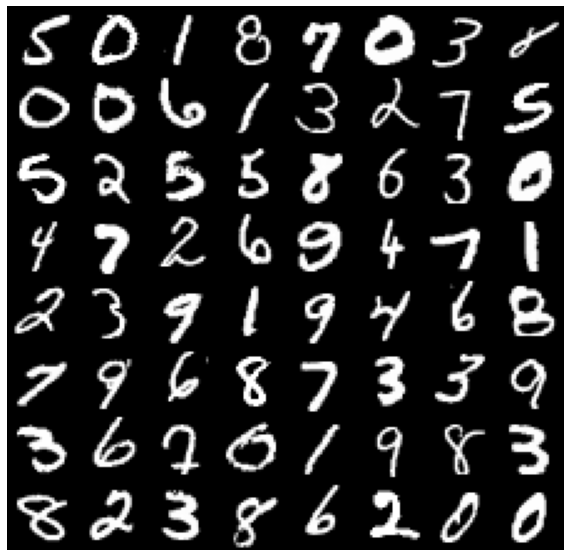
\includegraphics[width=0.4 \textwidth]{resources/minist_dataset.jpg}
		\caption{датасет рукописних цифр MNIST}
		\label{fig:minist_dataset}
	\end{figure}
	На її основі буде здійснюватись тренування моделі та аналіз атак.
	
	\section{Тренування моделі}
	\label{sec:model}
	\large{\textbf{TODO короткий опис реалізованої моделі}} \\
	% ============================================ %
	
	% ============================================ %
	\chapter{Методи атак}
	В цьому розділі будуть розглянуті деякі методи генерування змагальних зразків, які були реалізовані і протестовані на лінійній моделі натренованій в розділі \ref{sec:model}.
	
	Далі, під час опису будуть використовуватись такі позначення:
	\begin{itemize}
		\item $\boldsymbol{X}$ - це зображення, зазвичай це 3-D тензор (ширина $\times$ висота $\times$ глибина). В нашому випадку має розміри $(28 \times 28 \times 1)$ пікселей, яке складаеться з додатніх цілих чисел в межах $[0, 255]$.
		\item $\boldsymbol{X}^{*}$ - згенерований змагальний приклад для зображення $\boldsymbol{X}$
		\item $y_{true}$ - правильний клас для зображення $\boldsymbol{X}$.
		\item $J(\boldsymbol{X}, y)$ - штрафна функція моделі. Ваги моделі $\omega$ навмисно не будемо вказувати, вважатимемо їх сталими, як значення які будуть отримані з моделі машинного навчання. В нашому випадку штрафною функцією є функція кросс-ентропії \ref{eq:cross-entropy}. 
		\item $Clip_{\boldsymbol{X}, \varepsilon} \{ \boldsymbol{X}^{*} \}$ - функція яка виконує по-піксельне обрізання зображення $X^{*}$ так, щоб результат був в $L_{\infty}$ $\varepsilon $ - околі вхідного зображення $\boldsymbol{X}$. Рівняння для цього виглядає наступним чином:
		
		\begingroup
		\setlength{\abovedisplayskip}{0pt}
		\setlength{\belowdisplayskip}{0pt}
		\begin{align}
		\label{eq:clip}
		\resizebox{.9 \textwidth}{!} 
		{
			$
			Clip_{X, \varepsilon} \{ \boldsymbol{X}^{*} \}(x, y, z) = 
			min\Big\{ 255, \boldsymbol{X}(x, y, z) + \varepsilon, max \{ 0, \boldsymbol{X}(x, y, z) - \varepsilon, \boldsymbol{X}^{*}(x, y, z) \} \Big\}
			$,
		}
		\end{align}
		\endgroup

		де $\boldsymbol{X}(x, y, z)$ - це значення каналу $z$ зображення $\boldsymbol{X}$ з координатами $(x, y)$.
	\end{itemize}


	\section{FGSM}
	Одним з найпошириніших методів для генерування змагальних зразків машинного навчання є Fast Gradient Sign Method. В перше він був представлений в роботі \textcite{goodfellow2014explaining}. Ідея цього методу полягає в тому, щоб знайти такий adversarial приклад $x^{*}$ який максимізую функцію втрати $J(x^{*}, y)$ до певного $L_{\infty}$ обмеження. Цього можна досягти один раз використавши використавши зворотне поширення:
	\begin{equation}
	X^{*} = X + \varepsilon \cdot sign(\Delta_x J(x, y)),
	\end{equation}
	де $\varepsilon$ - деякий гіперпараметер.
	
	Для того щоб застосувати цей метод для логістичної регресії необхідно обчислити градієнт від функції кросс-ентропії \ref{eq:cross-entropy}. Для цього спочатку знайдемо похідну від $softmax$ функції:
	\begin{align*}
		z_i = \omega\tran x\ith + b; \quad
		\hat{y}_i = a_i = softmax(z_i); \quad
		softmax(z_i) = \frac{e^{z_i}}{\sum_{k=1}^{C} e_k^z}; \quad
	\end{align*}
	Якщо $i = j$,
	\begin{align}
	    \pdv{\hat{y_i}}{z_j} 
	    &=
	    \pdv{\frac{e^{z_i}}{\sum_{k=1}^{C} e_k^z}}{z_j} 
	    =
	    \frac{e^{z_i} \sum_{k=1}^{C} e^{z_k} - e^{z_j} e^{z_i}}{(\sum_{k=1}^{C}  e^{z_k})^2} 
	    = \\& =
	    \frac{e^{z_j}}{\sum_{k=1}^{C}  e^{z_k}} \times \frac{(\sum_{k=1}^{C} e^{z_k} - e^{z_j})}{\sum_{k=1}^{C}  e^{z_k}} 
	    = 
	    y_i(1-y_j)
	\end{align}
	Якщо $i \neq j$,
	\begin{align}
		\pdv{\hat{y_i}}{z_j}
		&=
		\pdv{\frac{e^{z_i}}{\sum_{k=1}^{C} e_k^z}}{z_j} 
		=
		\frac{0 - e^{z_j} e^{z_i}}{\sum_{k=1}^{C}  e^{z_k}} \times \frac{e^{z_i}}{\sum_{k=1}^{C} e^{z_k}} 
		= 
		-y_i y_j 
	\end{align}
	
	\begingroup
	\setlength{\abovedisplayskip}{0pt}
	\setlength{\belowdisplayskip}{0pt}
	
	Далі обчислюємо похідну від функції кросс-ентропії:
	\begin{align*}
		\xi(y, x) = - \sum_{i=1}^{C} y_i  \log (\hat{y_i})
	\end{align*}

	\begin{align*}
		\pdv{\xi}{z_i} 
		&= 
		- \sum_{j=1}^{C} \pdv{ y_j \log (\hat{y_j})}{z_i} 
		=
		- \sum_{j=1}^{C} y_j \pdv{ \log (\hat{y_j})}{z_i} 
		= 
		- \sum_{j=1}^{C} y_j \frac{1}{\hat{y_i}} \cdot \pdv{\hat{y_i}}{z_i} 
		= \\& =
		- \frac{y_i}{\hat{y_i}} \pdv{\hat{y_i}}{z_i} - \sum_{j \neq i} \frac{y_j}{\hat{y_j}} \pdv{\hat{y_j}}{z_i} 
		= 
		-\frac{y_i}{\hat{y_i}} \hat{y_i} (1 - \hat{y_i}) - \sum_{j \neq i} \frac{y_j}{\hat{y_j}} (-\hat{y_i} \hat{y_j}) 
		= \\& =
		-y_i + y_i \hat{y_i} + \sum_{j \neq i} y_j \hat{y_i}
		= 
		-y_i + \sum_{j=1}^{C} y_j \hat{y_i} 
		=
		\hat{y_i} - y_i ,
	\end{align*}
	\endgroup
	де i = 1, ..., C
	\newline	
	Тепер можна обчислити градієнт від штрафної функції по $x$:
	\begin{align}
		\pdv{\xi}{x_i} 
		&=
		\pdv{\xi}{z_i} \pdv{z_i}{x_i} 
		=
		(\hat{y_i} - y_i) \pdv{(\omega\tran x_i+ b)}{x_i} 
		=
		(\hat{y_i} - y_i) \omega\tran 
		=
		dz \cdot \omega\tran
	\end{align}
	 Маючи всі наведені обчислення, можна записати алгоритм знаходження змагального прикладу [\ref{alg:fgsm}].
	\begin{algorithm}
		\caption{$FGSM$}
		\label{alg:fgsm}
		\begin{algorithmic}[1]
			\State \algorithmicrequire{Приклад $x$, клас $y_{true}$, класифікатор $f$, параметри: $\omega, b$.}
			\State \algorithmicrequire{значення пертурбації $\varepsilon$.}
			\State \algorithmicensure{ Adversarial $x^{*}$ з нормою $\|x^{*} - x\|_{\infty} \leq \varepsilon $;}
			\State $z = \omega\tran x + b$;
			\State $\hat{y} = softmax(z)$;
			\State $\delta = (\hat{y} - y_{true}) \cdot \omega\tran$;
			\State $x^{*} = Clip_{X, \varepsilon} \big\{ x + \alpha \cdot sign( \delta ) \big\}$;
			\State \algorithmreturn{$x^{*} = x^{*}_{T}$}.
		\end{algorithmic}
	\end{algorithm}
	
	\section{I-FGSM}
	Даний метод є модифікацією попереднього, особливість якого полягає в тому, що для знахождення змагального прикладу буде використовуватись ітераційний підхід.	Ми застосовуємо звичайний метод декілька разів з певним невеликим кроком $a$ і після кожного кроку використовуємо функцію $clip$ \ref{eq:clip}, для того щоб переконатись що значення знаходяться в $\varepsilon$-околі оригінального зображення.

	Ітераційний алгоритм швидкого градієнтного спуску буде мати вигляд [\ref{alg:i-fgsm}].
	
	\begin{algorithm}
		\caption{$I-FGSM$}
		\label{alg:i-fgsm}
		\begin{algorithmic}[1]
			\State \algorithmicrequire{Приклад $x$, значення класу $y_{true}$, класифікатор $f$}
			\State \algorithmicrequire{значення пертурбації $\varepsilon$, кількість ітерації $T$.}
			\State \algorithmicensure{ Adversarial $x^{*}$ з нормою $\|x^{*} - x\|_{\infty} \leq \varepsilon $;}
			\State $a = \varepsilon / T $;
			\State $x^{*} = x$;
			\For{$t=0 \; to \; T-1$}
			\State $x^{*} = Clip_{X, \varepsilon} \big\{ x^{*} + \alpha \cdot  sign(\Delta_x J(x, y)) \big\}$;
			\EndFor
			\State \algorithmreturn{$x^{*} = x^{*}_{T}$}.
		\end{algorithmic}
	\end{algorithm}
		
	\newpage
	\section{TI-FGSM}
	TI-FGSM або як його ще часто називаюсь Projected Gradient Descent є націленою версією попереднього алгоритму, а отже він дає можливість обрати клас який має передбачити модель. Два попередні методи описаних вище намагалися максимізувати функцію втрати для правильного класу, не вказуючи яким буде неправильний класс. Цей метод - навпаки, мінімізує функцію втрати для деякого заданого неправильного класу. На сам алгоритм це вплине так, що на етапі додавання пертурбації у зображення знак буде змінений на протилежний.

	\begin{algorithm}
		\caption{$TI-FGSM$}
		\label{alg:ti-fgsm}
		\begin{algorithmic}[1]
			\State \algorithmicrequire{Приклад $x$, значення класу $y_{true}$, класифікатор $f$}
			\State \algorithmicrequire{значення пертурбації $\varepsilon$, кількість ітерації $T$.}
			\State \algorithmicensure{ Adversarial $x^{*}$ з нормою $\|x^{*} - x\|_{\infty} \leq \varepsilon $;}
			\State $a = \varepsilon / T $;
			\State $x^{*} = x$;
			\For{$t=0 \; to \; T-1$}
			\State $x^{*} = Clip_{X, \varepsilon} \big\{ x^{*} - \alpha \cdot  sign(\Delta_x J(x, y)) \big\}$;
			\EndFor
			\State \algorithmreturn{$x^{*} = x^{*}_{T}$}.
		\end{algorithmic}
	\end{algorithm}

	\section{MI-FGSM}	
	Попередні розглянуті методи хоч і є ефективними, але мають певні недоліки.
	Для прикладу однокроковий (FGSM), вираховує градієнт тільки один раз, припускаючи, що межа рішень є лінійною. На практиці це зазвичай не так і тому для змагального прикладу, згенерованого таким чином, характерне $"$недотренування$"$, що обмежує ефективність атаки. З іншого боку ітеративний метод (I-FGSM), з кожною ітерацією жадібно рухає змагальний приклад в напрямку градієнту, що може призвести до зупинки в локальнії точці оптимума та $"$перетренуванню$"$ моделі. Щоб вирішити цю проблему в роботі \textcite{dong2017boosting} була представленна momentum оптимізація ітеративного методу. Він допомагає стабілізувати напрямок зміни, прикладу що допомагає уникнути локального оптимума.
	\\{\textbf{TODO опис momentum метода}}  \\
	Алгоритм даної модифікації має наступний вигляд \ref{alg:mi-fgsm}	
	\begin{algorithm}
		\caption{$MI-FGSM$}
		\label{alg:mi-fgsm}
		\begin{algorithmic}[1]
			\State \algorithmicrequire{Приклад $x$, значення цілі y, класифікатор $f$.};
			\State \algorithmicrequire{значення пертурбації $\varepsilon$, значення цілі y, кількість ітерації $T$.};
			\State \algorithmicensure{ Adversarial $x^{*}$ з нормою $\|x^{*} - x\|_{inf} \leq \varepsilon $};
			\State $a = \varepsilon / T$;
			\State $g0 = 0;$ $x^{*}_0 = x$;
			\For{$t=0 \quad to \quad T-1$}
			\State $g_{t+1} = \mu \cdot g_t + \frac{\Delta_x J(x^{*}, y)}{\|\Delta_x J(x^{*}, y)\|_1}$;
			\State $x^{*} = Clip_{X, \varepsilon} \big\{ x^{*}_{t} + \alpha \cdot sign(g_{t+1}) \big\}$;
			\EndFor
			\State \algorithmreturn{$x^{*} = x^{*}_{T}$}.
		\end{algorithmic}
	\end{algorithm}
	
	\newpage
	\section{DeepFool}
	DeepFool була вперше представлена в роботі \textcite{moosavidezfooli2015deepfool}. На відмінно від FGSM методу цей алгоритм не можна використовуватись для націлених атак, де є можливість вибрати клас який має передбачити модель. Отже, його можна використовувати тільки для генерування прикладів які будуть класифікуватись відмінно від правильно класу. Основною метою цього методу є знаходження мінімального необхідного значення пертурбація, для того щоб модель хибно передбачила клас прикладу.
	
	\begin{figure}[h]
		\centering
		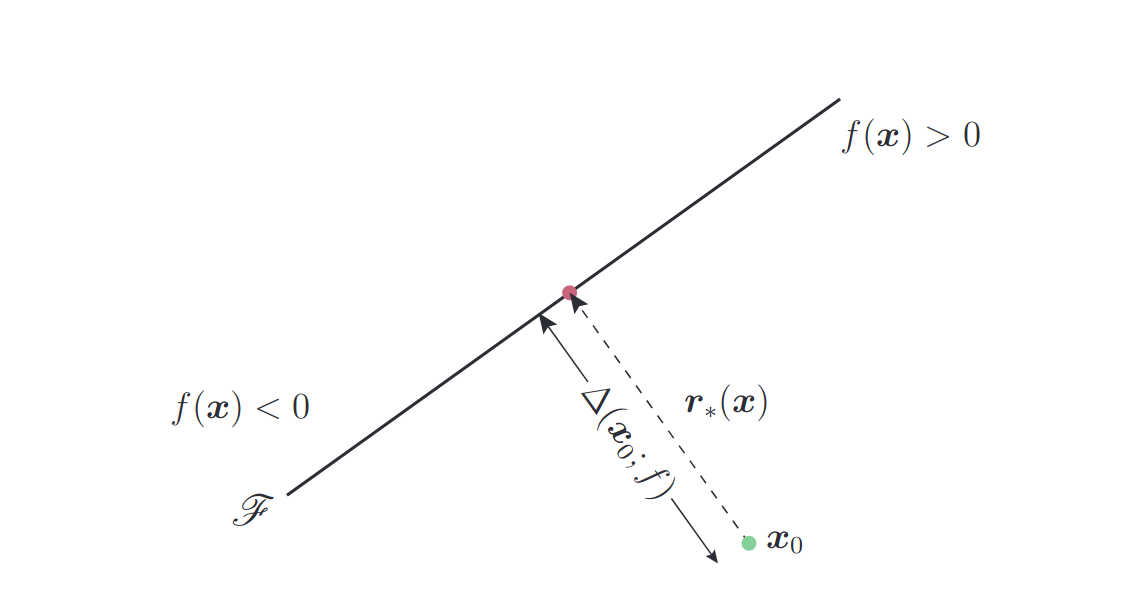
\includegraphics[width=\textwidth]{resources/deepfool.jpg}
		\caption{Приклад для лінійного бінарного класифікатора \cite{moosavidezfooli2015deepfool}}
		\label{fig:dfhyperline}
	\end{figure}

	Для випадку бінарної класифікації легко бачити, що надійність моделі $f$ в точці $ x_{0}, \; \Delta(x_{0}; f)$, дорівнює відстанні від $x_{0}$ до площини гіперпараметра $\mathscr{F} = \{ x: \omega\tran x + b = 0 \}$, яка розділяє два класи (Рис. \ref{fig:dfhyperline}). Таким чином, мінімальний зсув, необхідний для зміни рішення класифікатора відповідає ортогональній проекції $x_{0}$ на $\mathscr{F}$. Це можна записати у вигляді формули:
	\begin{align}
		r_{*}(x_{0}) := -\frac{f(x_{0})}{\norm{\omega}_{2}^{2}} \omega .
	\end{align}

	Для випалку $l_2$ норими DeepFool алгоритм для мультикласового випадку буде мати наступний вигляд [\ref{alg:deepfool}].

	\begin{algorithm}
		\caption{DeepFool: мультикласовий випадок}
		\label{alg:deepfool}
		\begin{algorithmic}[1]
			\State \algorithmicrequire{Приклад $x$, значення цілі y, класифікатор $f$.};
			\State \algorithmicrequire{значення цілі y, кількість ітерації $T$.};
			\State \algorithmicensure{ Adversarial $x^{*}$ з нормою $\|x^{*} - x\|_{2} \leq \varepsilon $};
			\State $x_0 = x$; $i = 0$; 
			\While{$\hat{f}(x_i) = \hat{f}(x_0) $}
				\For{$k \neq \hat{f}(x_0)$}
					\State $ w_{k}' = \Delta f_k(x_i) - \Delta f_{\hat{k}(x_0)} (x_i)$;
					\State $ f_{k}' = \Delta f_k(x_i) - \Delta f_{\hat{k}(x_0)} (x_i)$;
				\EndFor
				\State $\hat{l} = \arg \min_{k \neq \hat{f}(x_0)} \frac{\abs{f_{k}'}}{\|w_{k}'\|_2}$;
				\State $r_i = \frac{\abs{f_{\hat{l}}'}}{\|w_{\hat{l}}'\|_{2}^{2}} w_{\hat{l}}'$;
				\State $x_{i+1} = x_i + r_i$;
				\State $i = i + 1$;
			\EndWhile
			\State \algorithmreturn{$\hat{r} = \sum_{i} r_i $}.
		\end{algorithmic}
	\end{algorithm}
	

	Для того що реалізувати цей алгоритм необхідно спочатку знайти градієнт від функції кросс-ентропії \ref{eq:cross-entropy} по $x$.

	Маючи:
	\begin{equation}
		\pdv{\hat{y_i}}{x_k}  =
		\begin{cases}
		y_i(1-y_j) & \text{, якщо $i = j$}\\
		- y_i y_j & \text{, якщо $i \neq j$}\\
		\end{cases}
		\; \text{, де} \quad i = 1, .. ,C; \; j = 1, .. ,C;
	\end{equation}
	
	При знаходженні похідної нас цікавить випадок $i = j$, тому отримуємо:
	\begin{align*}
		\pdv{\hat{y_i}}{x_k} 
		&=
		\pdv{\hat{y_i}}{z_j} \pdv{z_j}{x_k} 
		=
		y_i(1-y_i) \pdv{(\omega\tran x_k + b)}{x_k} 
		=
		y_i(1-y_i) \omega\tran 
		=
		dz \cdot \omega\tran
	\end{align*}

	%\begin{lstlisting}[language=Python]
	%
	%\end{lstlisting}[language=Python]
	
	% ============================================ %	
	\chapter{Методи захисту}
	
	\section{Randomization}
	
	Одним з ефективних методів захисту, який добре себе продемонструва в ході змагань за найкращих метод атак та захисту 2018 року \cite{kurakin2018adversarial} є рандомізація вхідних даних.
	
	Зазвичай пертурбації, які генеруються в наслідок ітеративних атак, можуть легко опинитись перетренованими для деякий параметрів моделі і є унікальними для кожного прикладу. Ця властивість дає можливість зробити висновок, що трансформації додані до вхідних даних, такі як зміна роміру, стискання, або додавання відступів до зобаження може зруйнувати структуру певної змагальної пертурбації і таким чином стати непоганим захистом.
	Цей метод є ефективнним і для атак на відкриту модель теж, якщо трансформації відбуваються випадково, а нападник не знає про характер цих трансформації.	
	
	\section{Denoising}
	Ще одним з методів захисту є позбавлення від шуму вхідний даних.
	\\ \large{\textbf{TODO опис метода}} \\
	
	% ============================================ %	
	\chapter{Аналіз атак}
	\large{\textbf{TODO аналіз методів та захисту, графіки ефективності атак/захисту (Вже частково реалізовані)}}	\\
	% ============================================ %	


	\chapter{Висновок} 
	\large{\textbf{Висновок}} \\
	% ============================================ %

	\nocite{goodfellow2014explaining}
	\nocite{kurakin2016adversarial}
	\nocite{moosavidezfooli2015deepfool}
	\nocite{dong2017boosting}
	\nocite{dong2019benchmarking}
	\nocite{yuan2017adversarial}
	\nocite{kurakin2018adversarial}
	
	\printbibliography[title={Бібліографія}]
	%\printbibliography
	% ============================================ %
\end{document}